\documentclass[../../main.tex]{subfiles}
\graphicspath{{images/Beschleunigung/}{../../images/Beschleunigung/}}
\begin{document}
\subsection{Beschleunigung}
In diesem Kapitel wird auf die Implementierung der technischen Komponente 'Akustik' eingegangen.
\subsubsection{Anforderung}

\paragraph{Anforderungen}
\begin{itemize}
    \item Momentane Beschleunigung auslesen
      \subitem Fahrtrichtung
      \subitem Querbeschleunigung
    \item Beschleunigung in Geschwindigkeit und Distanz umrechnen
    \item Approximierte Position berechnen
    %\item (Optional) Zentrifugalkräfte in Kurven berechnen
\end{itemize}

\subsubsection{Lösung}
Die Lösung wird wie in PREN1 beschrieben, umgesetzt.

Der Beschleunigungssensor wird direkt an die 'Movement'-Klasse angebunden. Diese verarbeitet die erhaltenen Daten weiter zu Geschwindigkeit und Beschleunigung.

\paragraph{Technologien / Komponente}
Softwaretechnisch ist die Komponente in Python3 realisiert. Für die Umsetzung wird auf die Bibliotheken 'smbus2', 'time' und 'sys' zurückgegriffen. 'smbus2' enthält alle nötigen Informationen über den GPIO (General Purpose Input / Output) Bus. 'time' und 'sys' enthalten für die Entwicklung unterstützende Funktionen. 

\paragraph{Aufbau}
Der Sensor wird über die $I^2C$ Schnittstelle angesprochen und verwendet somit eine Datenleitung (SDA) und eine Clockleitung (SCL). Für die Stromversorgung werden die Anschlüsse für 3.3V des GPIO Headers benutzt.

\begin{table}[H]
  \begin{figure}[H] \centering
    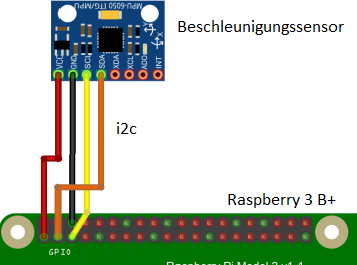
\includegraphics[width=0.33\textwidth]{Verkabelung_BeschlSensor}
    \caption{Verkabelung Beschleunigungssensor (http://fritzing.org)}
    \label{fig:Beschleunigungssensor}
  \end{figure}
  \begin{center}
  \begin{tabular}{lll}
  Bezeichnung     & GPIO Port & MPU 6050 \\ \hline
  Stromversorgung & 3V3      & VCC      \\ \hline
  Ground          & GND      & GND      \\ \hline
  Daten          & SDA      & SDA       \\ \hline
  Clock          & SCL      & SCL       \\ \hline
  \end{tabular}
  \end{center}
\end{table}

\paragraph{Prozessablauf}
Sobald die 'Movement' Komponente gestartet wird, liest diese im 50ms Takt Daten über den Beschleunigungssensor ein.

\paragraph{Soll-Ist-Vergleich}


\subsubsection{Entwicklungsablauf}


\subsubsection{Testing}

\subsubsection{Reflexion}

\end{document}